\chapter{Systematic Literature Review}
\label{ch:slr}

\section{Introduction}
\label{sec:slr-intro}

This chapter presents a systematic literature review (SLR) conducted to map
the state of the art at the intersection of process mining, stochastic
modeling, and machine learning applied to software process forecasting. The
review follows the guidelines established by Kitchenham and
Charters~\cite{kitchenham2007} for evidence-based software engineering,
complemented by the snowballing procedures described by
Wohlin~\cite{Wohlin2024} and the mapping study guidelines of Petersen et
al.~\cite{petersen2015}. The primary objective is to identify, classify, and
synthesize existing approaches that combine process-aware techniques with
predictive modeling for software development outcomes, establishing the
research gap that motivates PATHCAST proposed in
Chapter~\ref{ch:method}.

The review addresses three overarching research questions, each decomposed
into two sub-questions covering the application landscape of process mining in
SDLC contexts, the techniques and prediction methods employed, and the degree
of integration between process mining and stochastic forecasting methods.


\section{Review Protocol}
\label{sec:slr-protocol}

\subsection{Research Questions}
\label{sec:slr-rqs}

The SLR is guided by the following research questions, structured to
progressively map the landscape from application scope to technique
integration:

\begin{table}[htbp]
\centering
\caption{Research questions and expected outputs.}
\label{tab:slr-rqs}
\small
\setlength{\tabcolsep}{4pt}
\begin{tabular}{c c p{7.1cm} p{3.8cm}}
\toprule
\textbf{RQ} & \textbf{Sub-RQ} & \textbf{Question} & \textbf{Expected Output} \\
\midrule
RQ1 & RQ1.1 & Which SDLC phases have been analyzed with process mining? &
  Frequency distribution by phase \\
RQ1 & RQ1.2 & What event log sources are used and how are they constructed? &
  Taxonomy of sources and construction methods \\
\midrule
RQ2 & RQ2.1 & Which process discovery algorithms have been applied to SDLC? &
  Comparative matrix \\
RQ2 & RQ2.2 & Which predictive and stochastic techniques have been used? &
  Technique classification \\
\midrule
RQ3 & RQ3.1 & What is the level of integration between PM and stochastic
  methods? & Integration maturity assessment \\
RQ3 & RQ3.2 & What gaps exist for process-aware forecasting in the SDLC? &
  Gap analysis matrix \\
\bottomrule
\end{tabular}
\end{table}


\subsection{Search Strategy}
\label{sec:slr-search}

The search strategy combines automated database search with backward and
forward snowballing. The automated search targets five digital libraries:
IEEE~Xplore, ACM Digital Library, Scopus, Web of Science, and SpringerLink.

\subsubsection{PICO Decomposition}

The search string construction follows the PICO framework adapted for
software engineering, as shown in Table~\ref{tab:pico}.

\begin{table}[htbp]
\centering
\caption{PICO decomposition for search string construction.}
\label{tab:pico}
\begin{tabular}{lp{4cm}p{7cm}}
\toprule
\textbf{Facet} & \textbf{Role} & \textbf{Concepts} \\
\midrule
Population    & Application domain    & Software engineering, SDLC, software process,
                                        DevOps, CI/CD \\
Intervention  & Analytical technique  & Process mining, Markov chain, Monte Carlo,
                                        predictive PM, ML \\
Comparison    & N/A                   & (omitted) \\
Outcome       & Result                & Forecasting, prediction, lead time, cycle time,
                                        process model \\
\bottomrule
\end{tabular}
\end{table}

\subsubsection{Search Strings}

Three complementary search strings are executed to maximize coverage while
maintaining precision.

\paragraph{Principal String (P $\wedge$ I).}
Block~P captures the software engineering context:

\begin{quote}
\small
\texttt{("software engineering" OR "software development" OR "software process"
OR "software lifecycle" OR "software life cycle" OR "SDLC" OR "development
lifecycle" OR "development life cycle" OR "DevOps" OR "CI/CD" OR "continuous
integration" OR "continuous delivery" OR "agile development" OR "agile process"
OR "issue tracking" OR "bug tracking" OR "version control" OR "code review" OR
"pull request" OR "software project" OR "software repository" OR "software
maintenance" OR "software evolution")}
\end{quote}

Block~I captures the process mining and stochastic modeling techniques:

\begin{quote}
\small
\texttt{("process mining" OR "process discovery" OR "conformance checking" OR
"workflow mining" OR "predictive process monitoring" OR "process prediction" OR
"remaining time prediction" OR "process forecasting" OR "event log" OR "process
simulation" OR "Monte Carlo simulation" OR "Markov chain" OR "Markov model" OR
"stochastic process model" OR "transition probability" OR "absorbing chain" OR
"lead time prediction" OR "cycle time prediction")}
\end{quote}

\paragraph{Complementary String (MSR $\rightarrow$ Process Modeling).}
Captures studies using MSR terminology without canonical process mining terms:

\begin{quote}
\small
\texttt{("mining software repositories" OR "software repository mining" OR
"GitHub mining" OR "Jira mining") AND ("process model" OR "Markov" OR "Monte
Carlo" OR "stochastic" OR "lead time" OR "cycle time" OR "throughput" OR
"transition matrix")}
\end{quote}

\paragraph{Frontier String (Stochastic $\wedge$ PM $\wedge$ SE).}
Targets the intersection of stochastic methods with process mining in software
contexts:

\begin{quote}
\small
\texttt{("Monte Carlo" OR "Markov chain" OR "stochastic simulation" OR
"probabilistic forecast" OR "transition matrix") AND ("process mining" OR
"event log" OR "workflow mining" OR "process model" OR "business process") AND
("software development" OR "software engineering" OR "software process" OR
"DevOps" OR "SDLC" OR "issue tracker" OR "commit log" OR "build pipeline")}
\end{quote}

The strings are adapted to each database's syntax and field conventions as
summarized in Table~\ref{tab:db-adaptations}. The search scope covers
publications from January 1994 to December 2026.

\begin{table}[htbp]
\centering
\caption{Database-specific search adaptations and raw retrieval counts.}
\label{tab:db-adaptations}
\small
\setlength{\tabcolsep}{4pt}
\begin{tabular}{p{2.6cm} p{2.6cm} c p{5.0cm} r}
\toprule
\textbf{Database} & \textbf{Search Field} & \textbf{Strings} & \textbf{Filters} & \textbf{Records} \\
\midrule
Scopus         & TITLE-ABS-KEY & 3         & ar, cp; EN; 1994--2026                 & 2{,}377 \\
IEEE Xplore    & All Metadata  & 4 (split) & Conf.\ + Journals; 1994--2026          & 1{,}386 \\
Web of Science & TS (Topic)    & 3         & Article, Proc.; EN; 1994--2026         & 997 \\
SpringerLink   & Simplified    & 8 queries & Chapter, Article; EN                   & 2{,}884 \\
ACM DL         & Abstract      & 2         & Date: 1994--2026                       & 96 \\
Snowballing    & --            & --        & Backward + forward                     & 595 \\
Control set    & --            & --        & Manual                                 & 12 \\
\midrule
\textbf{Total} &  &  &  & \textbf{8{,}347} \\
\bottomrule
\end{tabular}
\end{table}

\subsubsection{Snowballing Procedure}

Backward snowballing examines the reference lists of all included primary
studies. Forward snowballing uses Google Scholar citation tracking to identify
subsequent works that cite the included studies. Both rounds apply the same
inclusion and exclusion criteria defined in Section~\ref{sec:slr-criteria}.

\subsubsection{Search String Validation}

The search strings are validated against a control set of 10 papers that are
known to be relevant to the review scope
(Table~\ref{tab:validation-set}). The acceptance threshold is $\geq 8/10$
papers found; the validation returned $10/10$ ($100\%$, PASS).

\begin{table}[htbp]
\centering
\caption{Control papers for search string validation.}
\label{tab:validation-set}
\small
\setlength{\tabcolsep}{4pt}
\begin{tabular}{c p{4.5cm} p{4.1cm} p{1.6cm}}
\toprule
\textbf{\#} & \textbf{Paper} & \textbf{Justification} & \textbf{Captured via} \\
\midrule
V1  & Cook \& Wolf (1998)            & Seminal PM + SE                    & ACM \\
V2  & Rubin et al. (2007)            & PM framework for SW processes      & Scopus \\
V3  & Poncin et al. (2011)           & PM + MSR intersection              & IEEE \\
V4  & Caldeira \& Cardoso (2019)     & PM + SW process assessment         & IEEE \\
V5  & Lemos et al. (2011)            & PM for SW process management       & IEEE \\
V6  & Whittaker \& Thomason (1994)   & Markov + SW testing (seminal)      & Scopus \\
V7  & Tax et al. (2017)              & PPM seminal (BPM baseline)         & Control \\
V8  & Rogge-Solti \& Weske (2015)    & Stochastic + PM forecasting        & Scopus \\
V9  & Rozinat et al. (2009)          & PM $\rightarrow$ Simulation bridge & Control \\
V10 & Gupta \& Sureka (2017)         & PM multi-repository in SE          & ACM \\
\bottomrule
\end{tabular}
\end{table}


\subsection{Inclusion and Exclusion Criteria}
\label{sec:slr-criteria}

The inclusion criteria are organized in two tiers. Formal criteria
(IC1--IC3) filter on publication attributes and are applied during the
database search configuration. Content criteria (IC4a--IC4d) require that the
study's research contribution addresses at least one of four specific
technique-domain intersections; they are applied during title/abstract and
full-text screening. Exclusion criteria (EC1--EC6) are applied cumulatively
across both screening phases.

\begin{table}[htbp]
\centering
\caption{Inclusion and exclusion criteria.}
\label{tab:criteria}
\small
\setlength{\tabcolsep}{4pt}
\begin{tabular}{c c p{10.2cm}}
\toprule
\textbf{Type} & \textbf{ID} & \textbf{Criterion} \\
\midrule
\multirow{7}{*}{Inclusion}
& IC1  & Publication period: 1994--2026 (from Whittaker \& Thomason onward). \\
& IC2  & Language: English. \\
& IC3  & Peer-reviewed journal article, conference paper, or workshop paper
          ($\geq$4 pages). \\
& IC4a & Applies process mining techniques (discovery, conformance checking,
          predictive process monitoring) to software development artifacts
          (commits, issues, pull requests, CI/CD logs, bug trackers, VCS). \\
& IC4b & Uses stochastic models (Markov chains, Monte Carlo, stochastic Petri
          nets, absorbing chains) to analyze software development processes or
          workflows. \\
& IC4c & Proposes or evaluates forecasting of software process metrics (lead
          time, cycle time, remaining time, throughput, defect rates) from
          event logs or repository data. \\
& IC4d & Mines software repositories (GitHub, Jira, VCS, CI/CD platforms) to
          discover, analyze, or improve software process models. \\
\midrule
\multirow{6}{*}{Exclusion}
& EC1  & Application domain is exclusively outside software development
          (healthcare, manufacturing, supply chain) without demonstrated
          relevance to SDLC processes. \\
& EC2  & Software appears only as the implementation platform; the process
          being analyzed is not a software development process. \\
& EC3  & Purely algorithmic or theoretical contribution without empirical
          evaluation in a software development context. \\
& EC4  & Secondary study (SLR, mapping study, survey) not specifically
          addressing PM or stochastic methods in software engineering. \\
& EC5  & Duplicate study (the most complete version is retained). \\
& EC6  & Full text inaccessible. \\
\bottomrule
\end{tabular}
\end{table}

At least one of IC4a--IC4d must be satisfied for inclusion. Criterion IC4b
ensures that seminal works applying Markov chains to software processes---such
as Whittaker and Thomason~\cite{whittaker1994}---are captured despite
predating the term ``process mining.''


\subsection{LLM-Assisted Screening Methodology}
\label{sec:slr-llm}

Given the scale of the working set (2{,}340 papers) and the requirement for
systematic, reproducible screening decisions with traceable rationale, the
title/abstract screening phase employs a language model as the primary
screener. Specifically, \textit{claude-haiku-4-5-20251001} is used via the
Anthropic Message Batches API, with a structured prompt encoding the IC4a--IC4d
and EC1--EC4 criteria, the PATHCAST scope description, and decision rules for
the three-class output: \texttt{include}, \texttt{exclude}, or \texttt{maybe}.

The screening prompt instructs the model to (i)~identify which ICs are
satisfied, (ii)~identify which ECs apply, (iii)~assign a decision with a
one-to-two sentence rationale, and (iv)~return the result as structured
JSON. The \texttt{maybe} class captures genuine uncertainty---typically
arising from missing abstracts or ambiguous domain terminology---without
forcing a binary decision.

At the full-text screening phase, the same model is applied with a stricter
prompt that enforces a binary outcome (\texttt{include} or \texttt{exclude})
with \texttt{pending} reserved only when the abstract is genuinely
insufficient for a decision.

This approach extends prior work on LLM-assisted systematic reviews
\cite{syriani2023,khraisha2024} to the software process mining domain. The
primary screener produces structured outputs that enable post-hoc quality
analysis. Human validation follows a two-stage protocol: (i)~all \texttt{include}
decisions are manually verified by the author; (ii)~a random 20\% sample of
\texttt{exclude} and \texttt{maybe} decisions is reviewed by an independent
second reader, with inter-rater agreement reported via Cohen's $\kappa$. A
threshold of $\kappa \geq 0.61$ (substantial agreement) is required before
the screening results are treated as final. Until this validation cycle is
fully completed, all synthesis statements derived from the current included
set are treated in this chapter as \textit{provisional but analytically
informative}.


\subsection{Quality Assessment}
\label{sec:slr-qa}

Each included study is assessed against a quality checklist adapted from
Dyb{\aa} and Dings{\o}yr~\cite{dyba2008}, with eight binary criteria:

\begin{table}[htbp]
\centering
\caption{Quality assessment checklist.}
\label{tab:qa}
\begin{tabular}{clc}
\toprule
\textbf{\#} & \textbf{Criterion} & \textbf{Score} \\
\midrule
QA1 & Are the research objectives clearly stated?                    & 0/1 \\
QA2 & Is the software engineering context described in detail?       & 0/1 \\
QA3 & Is the data source (event log) described reproducibly?         & 0/1 \\
QA4 & Is the PM or stochastic technique formally defined?            & 0/1 \\
QA5 & Are results validated empirically?                             & 0/1 \\
QA6 & Are threats to validity discussed?                             & 0/1 \\
QA7 & Is the study reproducible (data and/or code available)?        & 0/1 \\
QA8 & Are process model quality metrics reported (fitness, precision)?& 0/1 \\
\bottomrule
\end{tabular}
\end{table}

Studies scoring below 4.0/8 (50\%) are excluded from the synthesis. QA8
reflects the centrality of process model quality in the PATHCAST pipeline.

Table~\ref{tab:qa-results-placeholder} summarizes the current quality-assessment
results for the included set. QA has been applied to the first 76 provisionally
included studies identified in Round~1 of full-text screening; the 67 additional
studies confirmed in Round~2 are pending QA assessment.

\begin{table}[htbp]
\centering
\caption{Quality-assessment results for the current included set (143 total;
  QA applied to the first 76; 67 additional studies from Round~2 pending QA).}
\label{tab:qa-results-placeholder}
\begin{tabular}{lcp{6.5cm}}
\toprule
\textbf{QA Outcome} & \textbf{Count} & \textbf{Notes} \\
\midrule
Studies assessed (QA complete) & 76 & Round~1 confirmed set \\
Studies with score $\geq 4/8$ & 71 & Retained for synthesis \\
Studies with score $< 4/8$ & 5 & Excluded after QA \\
Mean QA score & 5.18 & Mean and standard deviation (1.13) \\
Median QA score & 5.00 & Median and interquartile range (4.00--6.00) \\
Studies pending QA & 67 & Round~2 confirmed (QA not yet applied) \\
\bottomrule
\end{tabular}
\end{table}


\subsection{Data Extraction}
\label{sec:slr-extraction}

For each included study, the attributes in Table~\ref{tab:extraction} are
extracted.

\begin{table}[htbp]
\centering
\caption{Data extraction form.}
\label{tab:extraction}
\small
\setlength{\tabcolsep}{4pt}
\begin{tabular}{p{3.6cm} p{8.1cm}}
\toprule
\textbf{Field} & \textbf{Description} \\
\midrule
ID                           & Unique identifier \\
Authors, Year, Venue         & Bibliographic metadata \\
SDLC Phase(s)                & Lifecycle phases covered \\
Event Log Source             & Jira, GitHub, GitLab, Jenkins, etc. \\
Event Log Construction       & Manual, semi-automatic, or automatic \\
PM Technique Category        & Discovery / Conformance / Enhancement / Prediction \\
Specific Algorithm(s)        & Alpha, Heuristics, Inductive Miner, etc. \\
Stochastic Method            & Markov / Monte Carlo / Stochastic Petri Net / None \\
ML Technique                 & RF, XGBoost, LSTM, etc. / None \\
Prediction Target            & Remaining time, outcome, lead time, delay, etc. \\
Integration Level            & L0 None / L1 Sequential / L2 Pipeline / L3 Unified \\
Validation Type              & Case study / Experiment / Industrial / Simulation \\
Tool/Platform                & PM4Py, ProM, Disco, custom, etc. \\
Dataset Size                 & Number of events and cases analyzed \\
Process Model Quality        & Fitness, precision, generalization (if reported) \\
\bottomrule
\end{tabular}
\end{table}


\section{Search Results and Study Selection}
\label{sec:slr-results-selection}

\subsection{Database Retrieval and Deduplication}

The three search strings executed across five databases returned 7{,}740
records. Backward and forward snowballing from the control set yielded an
additional 595 records. Together with 12 control papers maintained as a
validation-only set, the initial corpus totaled 8{,}347 records.
Table~\ref{tab:retrieval} summarizes the retrieval by source.

\begin{table}[htbp]
\centering
\caption{Record retrieval by source.}
\label{tab:retrieval}
\begin{tabular}{lrr}
\toprule
\textbf{Source} & \textbf{Raw Records} & \textbf{After Internal Dedup} \\
\midrule
Scopus (6 queries)      & 2{,}377 & 1{,}852 \\
SpringerLink (10 exports) & 2{,}884 & 1{,}543 \\
IEEE Xplore (manual)    & 1{,}386 & 1{,}263 \\
Snowballing             &   595   &   575   \\
Web of Science (4 queries) & 997  &   514   \\
ACM Digital Library (3 queries) & 96 &  34  \\
Control set (validation only) & 12 &    2   \\
\midrule
\textbf{Total} & \textbf{8{,}347} & \textbf{5{,}783} \\
\bottomrule
\end{tabular}
\end{table}

Cross-source deduplication removed 2{,}564 duplicate records (30.7\%),
yielding 5{,}781 unique primary-corpus papers plus 2 unique control papers.
Deduplication used normalized DOI matching, followed by fuzzy title matching
(Levenshtein similarity $\geq 0.9$) for records without DOIs.

\subsection{Operational Working Set Construction}

Screening 5{,}781 records in a single pass would require substantial
resources. A working set of 2{,}340 papers was therefore constructed from the
highest-signal primary queries---those whose query design directly targets the
PATHCAST intersection (process mining, stochastic modeling, and software
development)---as shown in Table~\ref{tab:working-set}. The remaining 3{,}441
records constitute a \textit{high-recall auxiliary corpus}, retained as a
frozen baseline and available for supplementary analysis if gaps in the
primary results warrant expansion.

\begin{table}[htbp]
\centering
\caption{Working set composition.}
\label{tab:working-set}
\small
\setlength{\tabcolsep}{4pt}
\begin{tabular}{p{2.2cm} p{8.3cm} r}
\toprule
\textbf{Database} & \textbf{Queries included} & \textbf{Unique papers} \\
\midrule
Scopus & scopus\_principal, scopus\_complementar, scopus\_fronteira,
         scopus\_markov\_testing, scopus\_stochastic\_petri,
         scopus\_simulation\_bridge & 2{,}197 \\
IEEE Xplore & ieee\_manual\_01 (PM + SE subgroup) & 97 \\
ACM DL & acm\_principal, acm\_msr & 46 \\
\midrule
\textbf{Total} & & \textbf{2{,}340} \\
\bottomrule
\end{tabular}
\end{table}

The working set preserves $10/10$ control papers when the validation-only
control set is included, and $8/10$ from primary queries alone---both above
the 80\% threshold.

\subsection{Title/Abstract Screening}

All 2{,}340 working-set papers were screened against IC4a--IC4d and EC1--EC4
using the LLM-assisted protocol described in Section~\ref{sec:slr-llm}. The
screening was executed across five sequential batches of up to 500 papers each
via the Anthropic Batches API, producing structured JSON outputs with decision,
rationale, and matched criteria for each record.

\begin{table}[htbp]
\centering
\caption{Title/abstract screening results.}
\label{tab:ta-screening}
\begin{tabular}{lrr}
\toprule
\textbf{Decision} & \textbf{Count} & \textbf{\%} \\
\midrule
Include & 111 & 4.7 \\
Maybe   & 775 & 33.1 \\
Exclude & 1{,}454 & 62.2 \\
\midrule
\textbf{Total} & \textbf{2{,}340} & 100.0 \\
\bottomrule
\end{tabular}
\end{table}

The \texttt{include} set (111 papers) and the \texttt{maybe} set (775 papers)
together form the full-text review queue of 886 papers. The
\texttt{exclude} decisions were driven primarily by EC1 (domain outside
software development, principally generic business process management) and EC3
(theoretical algorithm proposals without SE evaluation).

\subsection{Full-Text Screening}

The 886 papers forwarded from the T/A phase were subjected to LLM-assisted
full-text screening using the strict prompt described in
Section~\ref{sec:slr-llm} (decisions limited to \texttt{include},
\texttt{exclude}, or \texttt{pending}; \texttt{maybe} is not permitted at this
stage). To maximise the number of papers assessable by the LLM, a
multi-source abstract-enrichment cascade was executed prior to
screening---combining DOI-based lookups via Semantic Scholar, OpenAlex, CORE,
and Crossref, followed by title-based fallback lookups---raising abstract
coverage from 16.6\% to 72.6\% (643 of 886 papers).\footnote{Papers were
  processed in order of a five-band priority scheme: Band~A (91 papers,
  T/A \texttt{include} $\geq$2 ICs), Band~B (20, T/A \texttt{include} 1~IC),
  Band~C (39, T/A \texttt{maybe} + abstract), Band~D (152, T/A \texttt{maybe}
  + IC signal, no abstract), Band~E (584, T/A \texttt{maybe}, no IC signal, no
  abstract). Abstract enrichment and LLM re-screening were applied to Bands~A,
  B, C, and the subset of D/E that gained an abstract after enrichment.}

Table~\ref{tab:ft-screening} summarises the outcome.

\begin{table}[htbp]
\centering
\caption{Full-text screening outcomes (886 papers forwarded from T/A phase).}
\label{tab:ft-screening}
\begin{tabular}{lrr}
\toprule
\textbf{Outcome} & \textbf{Count} & \textbf{\%} \\
\midrule
Provisionally included & 143 & 16.1 \\
Excluded               & 497 & 56.1 \\
Pending (abstract insufficient for decision) & 2 & 0.2 \\
Without full-text access (manual review pending) & 244 & 27.5 \\
\midrule
\textbf{Total} & \textbf{886} & 100.0 \\
\bottomrule
\end{tabular}
\end{table}

Among the 497 excluded papers, EC3 (theoretical contribution without SE
evaluation) accounted for 44.1\% and EC1 (domain outside software
development) for 38.0\%; EC2 and EC4 together cover the remaining 17.9\%.
The 246 unresolved cases---244 papers for which a full-text copy could not be
obtained and 2 with abstracts that remained insufficient for a confident
decision---will be resolved through manual review or title-based exclusion
judgement. The final corpus is expected to comprise between 160 and 180
primary studies after these cases are resolved and QA consolidation is
complete (Section~\ref{sec:slr-qa}).

Figure~\ref{fig:prisma} presents the complete PRISMA 2020 flow
diagram~\cite{page2021} of the selection process.

\begin{figure}[p]
\centering
\begin{tikzpicture}[
  %% Main flow boxes (centre column) --- progressively narrower for funnel feel
  stg/.style={draw, rounded corners=4pt, align=center,
              text width=#1, minimum height=1.1cm,
              font=\small, fill=white, thick},
  stg/.default=8cm,
  %% Exclusion / note boxes (right column)
  exc/.style={draw, rounded corners=4pt, align=left,
              inner xsep=5pt, inner ysep=4pt,
              text width=5.0cm, minimum height=0.9cm,
              font=\footnotesize, fill=gray!8, draw=gray!60},
  %% Phase labels (left column)
  lbl/.style={font=\footnotesize\bfseries, text=gray!70,
              rotate=90, anchor=center},
  arr/.style={->, >=Stealth, thick},
  sidearr/.style={->, >=Stealth, dashed, draw=gray!70, thick},
]

%% -- PHASE: IDENTIFICATION ----------------------------------------------

\node[lbl] at (-6.8,-1.1) {IDENTIFICATION};
\draw[gray!40, dashed] (-6.0,-2.4) -- (-6.0, 0.2);

\node[stg=9.5cm, minimum height=1.3cm] (id) at (-0.5,0)
  {\textbf{Records identified} ($n = 8{,}347$)\\[3pt]
   Scopus~2{,}377 \textbullet{} \mbox{SpringerLink}~2{,}884\\
   IEEE~1{,}386 \textbullet{} WoS~997 \textbullet{} ACM~96\\[2pt]
   Snowballing~595 \textbullet{} Control~12};

\node[stg=9.5cm] (dedup) at (-0.5,-2.2)
  {\textbf{After cross-source deduplication} ($n = 5{,}783$)\\[3pt]
   2{,}564 duplicates removed (30.7\%)};

\draw[arr] (id) -- (dedup);

%% -- PHASE: SCREENING ----------------------------------------------------

\node[lbl] at (-6.8,-5.6) {SCREENING};
\draw[gray!40, dashed] (-6.0,-2.4) -- (-6.0,-8.0);

\node[stg=7.5cm, minimum height=1.2cm] (ws) at (-0.5,-4.5)
  {\textbf{Operational working set} ($n = 2{,}340$)\\[3pt]
   Scopus~2{,}197 \textbullet{} IEEE~97 \textbullet{} ACM~46};

\node[exc] (wsdrop) at (6.0,-4.5)
  {Deferred to auxiliary\\high-recall corpus ($n = 3{,}441$):\\
   \mbox{SpringerLink}, WoS,\\Snowball, extra IEEE/ACM};

\draw[arr] (dedup) -- (ws);
\draw[sidearr] (ws.east) -- (wsdrop.west);

\node[stg=7.5cm, minimum height=1.2cm] (ta) at (-0.5,-7.0)
  {\textbf{Title/Abstract screened} ($n = 2{,}340$)\\[3pt]
   LLM-assisted (Claude Haiku 4.5)};

\node[exc] (taexc) at (6.0,-7.0)
  {Excluded at T/A ($n = 1{,}454$)\\
   EC1: non-SE domain (BPM)\\
   EC3: theoretical, no SE eval.};

\draw[arr] (ws) -- (ta);
\draw[sidearr] (ta.east) -- (taexc.west);

%% -- PHASE: ELIGIBILITY --------------------------------------------------

\node[lbl] at (-6.8,-10.8) {ELIGIBILITY};
\draw[gray!40, dashed] (-6.0,-8.0) -- (-6.0,-13.6);

\node[stg=7cm, minimum height=1.3cm] (ftq) at (-0.5,-9.4)
  {\textbf{Full-text review queue} ($n = 886$)\\[3pt]
   T/A include~111 \textbullet{} T/A maybe~775\\
   Bands~A--E by priority};

\draw[arr] (ta) -- (ftq);

\node[stg=7cm, minimum height=1.4cm] (ft) at (-0.5,-12.2)
  {\textbf{Full-text screened (LLM)} ($n = 642$)\\[3pt]
   2~rounds \textbullet{} abstract coverage 72.6\%\\
   244 papers without FT decision};

\node[exc] (ftexc) at (6.0,-11.6)
  {Excluded at FT ($n = 497$)\\
   EC3: 219 (44.1\%) no SE eval.\\
   EC1: 189 (38.0\%) non-SE\\
   EC2: 106 \textbullet{} EC4: 24\\[3pt]
   FT pending ($n = 2$)\\
   Pending manual rev.\ ($n = 244$)};

\draw[arr] (ftq) -- (ft);
\draw[sidearr] (ft.east) -- (ftexc.west);

%% -- PHASE: INCLUDED ----------------------------------------------------

\node[lbl] at (-6.8,-14.6) {INCLUDED};
\draw[gray!40, dashed] (-6.0,-13.6) -- (-6.0,-15.6);

\node[stg=8cm, minimum height=1.3cm] (inc) at (-0.5,-14.8)
  {\textbf{\mbox{Provisionally included}} ($n = 143$)\\[3pt]
   +~3 pending manual review \textbullet{} Expected final: 160--180};

\draw[arr] (ft) -- (inc);

\end{tikzpicture}
\caption{PRISMA 2020 flow diagram of the study selection process.
  Phase labels follow the four-stage structure: Identification, Screening,
  Eligibility, and Included.}
\label{fig:prisma}
\end{figure}


\section{Results and Synthesis}
\label{sec:slr-synthesis}

\subsection{Preliminary Overview of Included Studies}

The current provisional set of 143 primary studies spans three decades
(1995--2026), with a clear acceleration from 2014 onward
(Figure~\ref{fig:year-dist}). Seventy percent of provisionally confirmed papers were
published between 2015 and 2026, reflecting the maturation of open-source
process mining toolkits (PM4Py, ProM) and the broader adoption of deep
learning frameworks in software engineering research.

\begin{figure}[htbp]
\centering
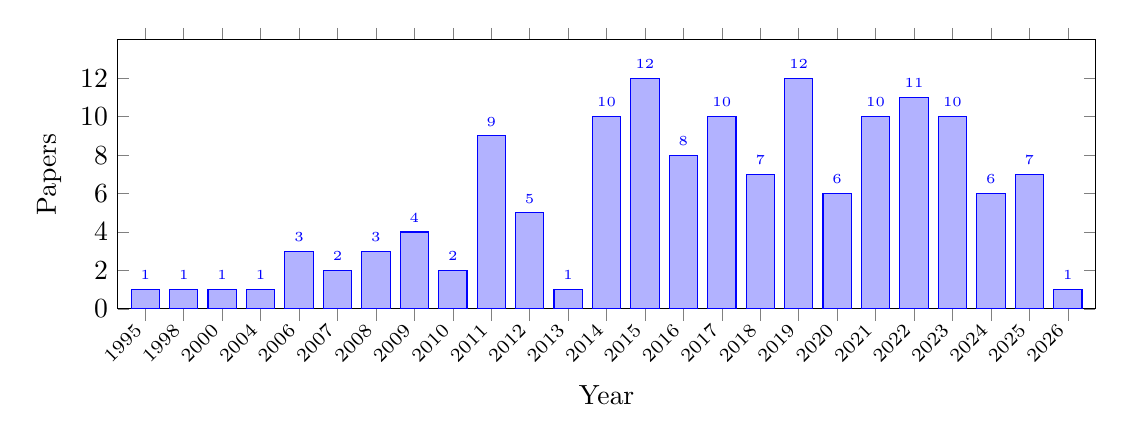
\begin{tikzpicture}
\begin{axis}[
  ybar,
  bar width=0.36cm,
  width=14cm, height=5cm,
  xlabel={Year},
  ylabel={Papers},
  xtick=data,
  xticklabels={1995,1998,2000,2004,2006,2007,2008,2009,2010,2011,2012,2013,2014,2015,2016,2017,2018,2019,2020,2021,2022,2023,2024,2025,2026},
  x tick label style={rotate=45, anchor=east, font=\scriptsize},
  ymin=0, ymax=14,
  ytick={0,2,4,6,8,10,12},
  enlarge x limits=0.03,
  fill=gray!40,
  draw=black,
  nodes near coords,
  nodes near coords style={font=\tiny, above},
]
\addplot coordinates {
  (1,1)(2,1)(3,1)(4,1)(5,3)(6,2)(7,3)(8,4)(9,2)(10,9)(11,5)(12,1)(13,10)(14,12)(15,8)(16,10)(17,7)(18,12)(19,6)(20,10)(21,11)(22,10)(23,6)(24,7)(25,1)
};
\end{axis}
\end{tikzpicture}
\caption{Distribution of provisionally confirmed studies by publication year
  ($n = 143$).}
\label{fig:year-dist}
\end{figure}

By document type, 107 papers (74.8\%) are conference papers, 31 (21.7\%)
are journal articles, and 5 are chapters or reviews. By source database,
Scopus contributed 96 provisionally confirmed inclusions, IEEE~Xplore 34,
and ACM~DL 13. The three papers pending manual full-text review are from the
Scopus corpus.

\subsection{Preliminary Criterion Coverage}

Figure~\ref{fig:ic-dist} shows the distribution of inclusion criteria among
the 143 provisionally confirmed papers (criteria are non-exclusive; a paper may satisfy
multiple).

\begin{figure}[htbp]
\centering
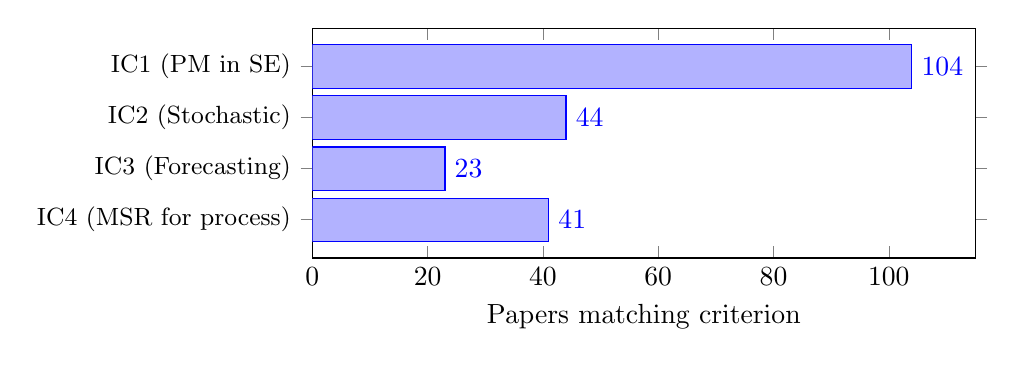
\begin{tikzpicture}
\begin{axis}[
  xbar,
  bar width=0.55cm,
  width=10cm, height=4.5cm,
  xlabel={Papers matching criterion},
  symbolic y coords={IC4 (MSR for process), IC3 (Forecasting), IC2 (Stochastic), IC1 (PM in SE)},
  ytick=data,
  y tick label style={font=\small},
  xmin=0, xmax=115,
  nodes near coords,
  nodes near coords align={horizontal},
  fill=gray!40,
  draw=black,
  enlarge y limits=0.25,
]
\addplot coordinates {
  (104,{IC1 (PM in SE)})
  (44,{IC2 (Stochastic)})
  (23,{IC3 (Forecasting)})
  (41,{IC4 (MSR for process)})
};
\end{axis}
\end{tikzpicture}
\caption{Inclusion criteria matched by the provisionally confirmed set ($n = 143$;
  non-exclusive; IC labels map to IC4a--IC4d in the protocol).}
\label{fig:ic-dist}
\end{figure}

IC1/IC4a (process mining applied to SE artifacts) is the dominant criterion,
matched by 104 papers (72.7\%). IC4/IC4d (repository mining for process modeling)
is second at 41 papers (28.7\%), reflecting the MSR community's overlapping
contributions. IC2/IC4b (stochastic modeling) appears in 44 papers (30.8\%) and
IC3/IC4c (forecasting of process metrics) in 23 papers (16.1\%). Notably, 56
papers (39.2\%) match IC1 only, without stochastic or forecasting components,
providing direct empirical evidence for the ``Descriptive Ceiling'' identified
in Finding~F1 below.

\subsection{Prevalent Exclusion Patterns}

Among the 497 FT-excluded papers, the dominant exclusion reason is EC3
(theoretical algorithm contributions without SE evaluation, $n \approx 219$,
44.1\%), indicating a substantial body of process mining and stochastic
modeling research that has not been empirically applied to software engineering
contexts. EC1 (domain exclusively outside software development, $n \approx 189$,
38.0\%), primarily generic business process management (BPM) studies that use
the same terminology as the search strings but apply techniques to
organizational processes unrelated to SDLC, is the second-largest reason. EC2
(software as implementation tool, not studied process, $n = 106$, 21.3\%) and
EC4 (out-of-scope secondary study, $n = 24$, 4.8\%) account for the remainder.
Note that EC counts sum above 497 as some papers triggered multiple exclusion
criteria. These patterns directly support Findings F3 and F4 below.

\subsection{PDF-Based Enrichment of the Confirmed Set}
\label{sec:slr-pdf-enrichment}

To reduce the number of placeholders in the synthesis while the final manual
full-text pass is still being completed, an article-level reading sheet was
generated for an \textit{opportunistic analytical subset} of studies whose
PDFs were locally available and machine-readable. This enrichment sample comprises
\textbf{73 papers}, each annotated with title, DOI, abstract, result summary,
relevance to the SLR, method family, type of evidence, and explicit
threats/limitations. A second operational pass then extended the extraction
table with SLR-oriented decision support columns: \textit{include/exclude},
reason for decision, RQ coverage, IC/EC criteria triggered, SDLC phase,
integration level (L0--L3), and reading priority. The reading sheets were
generated semi-automatically from the full PDFs and then consolidated into a
structured extraction table.

Of these 73 PDFs, the intended analytical frame is the current included set:
they correspond to the studies for which a locally accessible and
machine-readable full text was available at the time of analysis. The subset
therefore functions as a practical analytical view over the current included
material, not as an independent selection stage.

This enrichment sample is not used to change the PRISMA counts, redefine the
formal inclusion set, or replace the planned structured extraction of the
final included studies. Instead, it serves strictly as a triangulation layer
to refine provisional interpretations of RQ1--RQ3 with evidence grounded in
the full text rather than in title/abstract screening alone. The counts
reported in the following subsections therefore refer explicitly to the
\textbf{73 analyzed PDFs}, whereas the PRISMA flow and the selection
statistics continue to refer to the broader set of \textbf{143 provisionally
confirmed studies} plus \textbf{3 pending manual reviews}.

The operational pass classified \textbf{54 papers as include}, \textbf{13 as
maybe}, and \textbf{6 as exclude}. This does not override the formal
screening decisions already reported in the PRISMA flow; rather, it provides a
replicable prioritization layer for the final manual review and extraction of
evidence from the PDF subset only. Figure~\ref{fig:pdf-decision-dist}
summarizes this operational triage profile.

\begin{figure}[tbp]
\centering
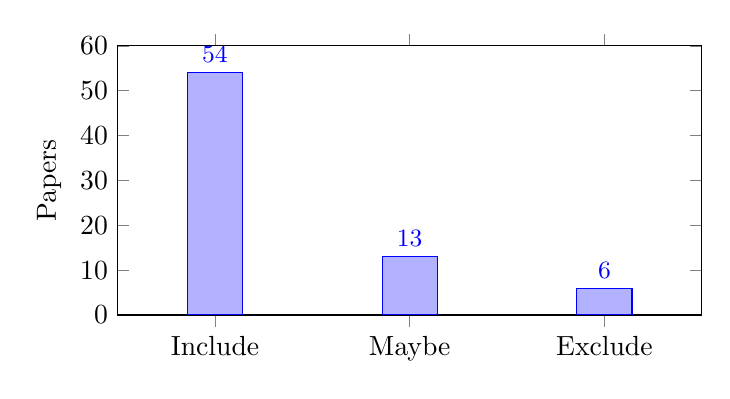
\begin{tikzpicture}
\begin{axis}[
  ybar,
  bar width=0.7cm,
  width=9cm, height=5cm,
  ylabel={Papers},
  symbolic x coords={Include,Maybe,Exclude},
  xtick=data,
  ymin=0, ymax=60,
  ytick={0,10,20,30,40,50,60},
  nodes near coords,
  nodes near coords style={font=\small, above},
  fill=gray!45,
  draw=black,
  enlarge x limits=0.25,
]
\addplot coordinates {(Include,54) (Maybe,13) (Exclude,6)};
\end{axis}
\end{tikzpicture}
\caption{Operational decision distribution in the 73-paper PDF enrichment subset.}
\label{fig:pdf-decision-dist}
\end{figure}

\subsection{RQ1: Application Landscape}
\label{sec:slr-rq1}

\subsubsection{RQ1.1: SDLC Phases Covered}

The PDF-based enrichment confirms an uneven coverage of the SDLC. Among the
73 analyzed full papers, \textbf{quality-related activities} (testing, defect
handling, review, and process evaluation) appear in 28 papers (38.4\%),
\textbf{development activities} (coding, commits, pull requests, repository
evolution) in 22 papers (30.1\%), and \textbf{delivery/DevOps contexts}
(CI/CD, build and release pipelines) in 19 papers (26.0\%). In contrast,
\textbf{design/architecture} appears in 10 papers (13.7\%) and
\textbf{requirements engineering} in only 7 (9.6\%).

This reinforces two conclusions. First, the literature is heavily concentrated
on phases where digital traces are abundant and already timestamped, such as
commits, issues, test events, and pipeline executions. Second, the early
SDLC phases remain structurally underrepresented, which weakens the ability
of current approaches to support end-to-end forecasting from requirements to
delivery. For PATHCAST, this supports a pragmatic focus on operational phases
with reliable event data while leaving room for future extensions toward
requirements and design logs.

The operational classification leads to the same conclusion from another
angle. Only a small minority of papers are centered on early lifecycle stages
such as requirements and design, while the bulk of high-priority readings is
concentrated on development, quality/testing, and delivery/DevOps settings.

\subsubsection{RQ1.2: Event Log Sources and Construction}

The enriched reading sheets show that event logs are constructed primarily
from three source families: \textbf{issue tracking systems} (especially Jira
and GitHub Issues), \textbf{version-control repositories} (Git/GitHub/SVN),
and \textbf{CI/CD or build pipelines}. A smaller but important subset uses
IDE interaction logs and educational development environments to capture
fine-grained coding behavior. Across the sample, the common pattern is not a
native event log but rather a \emph{derived} event log assembled from
repository metadata, commit histories, issue transitions, and pipeline
records.

The dominant construction problem is case correlation across tools. Studies
frequently analyze one source in isolation or perform ad hoc joins between
issues and commits, which limits reproducibility. This confirms that event-log
construction is not a preparatory detail but a central methodological layer in
software process mining. The finding directly justifies Stage~1 of PATHCAST as
an explicit transformation pipeline rather than an implicit data-cleaning step.

In the operational extraction, the most frequent data-source labels were
\textbf{IDE logs} (24 papers), followed by explicit \textbf{repository/VCS}
traces and combinations of repositories with issue trackers or CI/CD sources.
Seventeen papers still required manual inspection to determine the precise
origin of the data, which itself is evidence of incomplete reporting in the
literature.


\subsection{RQ2: Techniques and Prediction}
\label{sec:slr-rq2}

\subsubsection{RQ2.1: Discovery Algorithms Applied to SDLC}

The 73-paper enrichment indicates that \textbf{process mining remains the
dominant analytical family}, appearing in 42 papers in the form of discovery,
conformance checking, or process-oriented repository analysis. At this stage
of the review, the literature is much richer in \emph{process representation}
than in probabilistic forecasting. Several papers focus on discovering actual
flows, identifying deviations, bottlenecks, or collaboration patterns, but do
not operationalize those models into predictive engines.

The practical implication is that SDLC-oriented process mining is already
mature enough to describe and diagnose software processes, but not yet mature
enough to support a standardized forecasting stack. This is precisely the
transition that PATHCAST targets: moving from discovered process structures to
state-based probabilistic forecasting.

The more operational \texttt{técnica principal} coding shows the same pattern:
\textbf{40 papers} are led by process mining, while the remaining studies are
distributed across IA/NLP-based approaches (11), Markov chains (7),
simulation (6), and stochastic Petri nets (5). This confirms that the
forecasting literature remains fragmented across adjacent technique families
rather than consolidated around a single process-aware predictive paradigm, as
shown in Figure~\ref{fig:pdf-technique-dist}.

\begin{figure}[tbp]
\centering
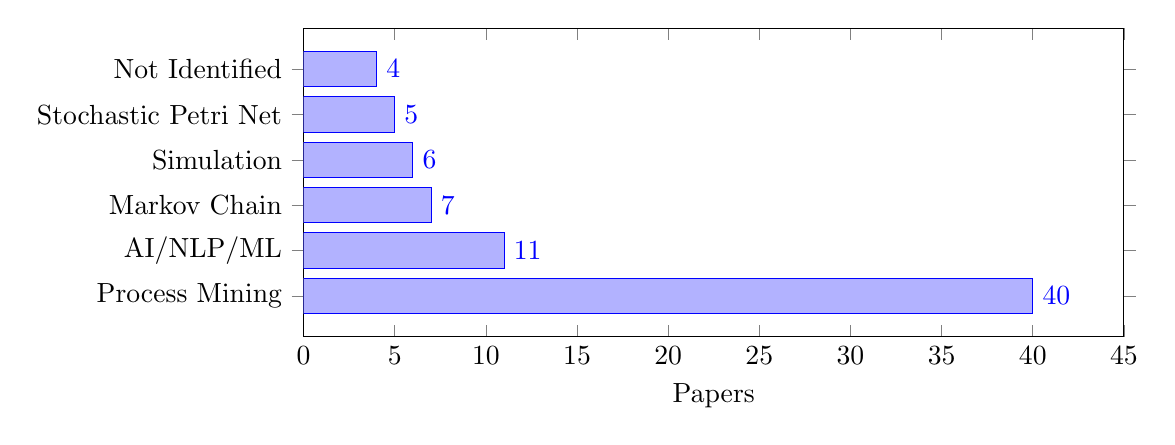
\begin{tikzpicture}
\begin{axis}[
  xbar,
  bar width=0.45cm,
  width=12cm, height=5.5cm,
  xlabel={Papers},
  symbolic y coords={Process Mining,AI/NLP/ML,Markov Chain,Simulation,Stochastic Petri Net,Not Identified},
  ytick=data,
  xmin=0, xmax=45,
  nodes near coords,
  nodes near coords align={horizontal},
  fill=gray!45,
  draw=black,
  enlarge y limits=0.18,
]
\addplot coordinates {
  (40,{Process Mining})
  (11,{AI/NLP/ML})
  (7,{Markov Chain})
  (6,{Simulation})
  (5,{Stochastic Petri Net})
  (4,{Not Identified})
};
\end{axis}
\end{tikzpicture}
\caption{Main technique families identified in the 73-paper PDF enrichment subset.}
\label{fig:pdf-technique-dist}
\end{figure}

\subsubsection{RQ2.2: Predictive and Stochastic Techniques}

The PDF analysis sharpens the stochastic-method picture. Among the 73 analyzed
papers, \textbf{9} explicitly use \textbf{Markov chains}, \textbf{9} use
\textbf{simulation-based approaches}, and \textbf{7} use \textbf{stochastic
Petri nets}. Typical targets include remaining time, duration or risk
estimation, delivery probability, collaboration-state evolution, and
process-performance evaluation. Representative examples include
\emph{Assessing the Risk of Software Development in Agile Methodologies Using
Simulation}, \emph{Exploring Collaboration Patterns in GitHub Using Discrete
Time Markov Chain}, and \emph{A Stochastic Petri net Model of Continuous
Integration and Continuous Delivery}.

However, the overlap between process mining and stochastic modeling is still
small. Only \textbf{5 of the 73 analyzed papers} simultaneously exhibit
explicit process-mining and stochastic components, and even these cases
typically stop at simulation or conformance analysis rather than advancing to
multi-stage forecasting with learned residual correction. This keeps the
review's central conclusion unchanged: the literature contains the
\emph{ingredients} of PATHCAST, but not their full composition.

From the perspective of research-question coverage, the operational sheet
shows that the sample is concentrated on \textbf{RQ2}. Twenty-two papers are
classified as primarily answering RQ2, and another 21 jointly address
\textbf{RQ1 + RQ2}. Only eight papers fall into \textbf{RQ2 + RQ3} and seven
into \textbf{RQ1 + RQ2 + RQ3}, which indicates that explicitly integrated
studies remain scarce even among the strongest candidates.


\subsection{RQ3: Integration and Gaps}
\label{sec:slr-rq3}

\subsubsection{RQ3.1: PM and Stochastic Integration Level}

The enriched full-paper sample indicates that most studies remain in the lower
integration levels. A large majority of the 73 analyzed papers fit either
\textbf{L0} (single-technique or contextual study without explicit
cross-technique chaining) or \textbf{L1} (two analytical layers are present,
but not yet composed as a reproducible end-to-end pipeline). Only a very
small subset approaches \textbf{L2}, where mined process structures and
stochastic behavior are linked in a semi-coherent pipeline.

No analyzed paper reaches \textbf{L3}, that is, a unified architecture
combining event-log construction, process mining, state-transition modeling,
Monte Carlo forecasting, and machine-learning enhancement under explicit
inter-stage contracts. This absence is not merely architectural; it also
reveals a validation gap, since most studies evaluate only one analytical
layer at a time.

The operational coding quantifies this more explicitly: \textbf{54 papers}
were classified as \textbf{L1}, \textbf{13 as L0}, and only \textbf{6 as L2}.
\textbf{No paper} reached \textbf{L3}. Even allowing for the heuristic nature
of the coding, the result is robust enough to support the central claim that
the literature has many partial bridges but no end-to-end process-aware
forecasting architecture for SDLC data. Figure~\ref{fig:pdf-integration-priority}
also juxtaposes this pattern with the reading-priority distribution, which is
useful for planning the next manual extraction round.

\begin{figure}[p]
\centering
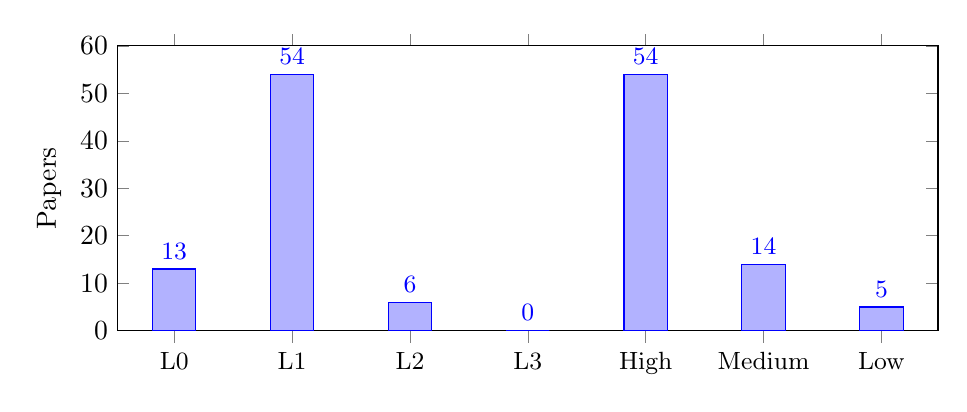
\begin{tikzpicture}
\begin{axis}[
  ybar,
  bar width=0.55cm,
  width=12cm, height=5.2cm,
  ylabel={Papers},
  symbolic x coords={L0,L1,L2,L3,High,Medium,Low},
  xtick=data,
  x tick label style={font=\small},
  ymin=0, ymax=60,
  ytick={0,10,20,30,40,50,60},
  nodes near coords,
  nodes near coords style={font=\small, above},
  fill=gray!45,
  draw=black,
  enlarge x limits=0.08,
]
\addplot coordinates {(L0,13) (L1,54) (L2,6) (L3,0) (High,54) (Medium,14) (Low,5)};
\end{axis}
\end{tikzpicture}
\caption{Operational integration levels and reading-priority distribution in the 73-paper PDF enrichment subset.}
\label{fig:pdf-integration-priority}
\end{figure}

\subsubsection{RQ3.2: Gap Analysis}

The PDF-based enrichment makes the gap structure more concrete. First, the
field remains \textbf{descriptively strong but forecastively weak}: many
studies can discover and assess process behavior, but few estimate future
paths or probabilistic completion distributions. Second, \textbf{evidence is
still method-heavy}: 39 of the 73 analyzed papers (53.4\%) are best
characterized as methodological proposals with limited empirical evidence,
while only 13 (17.8\%) report studies with clearly real-world data and 11
(15.1\%) present explicit experimental evaluations. Third, the most frequent
limitations in the sample are \textbf{dependence on modeling assumptions}
(56 papers) and \textbf{sensitivity to data/log quality} (19 papers),
followed by restricted empirical scope (16 papers).

Taken together, these patterns explain why PATHCAST requires both a formal
pipeline and an evaluation strategy grounded in real SDLC traces. The gap is
not the absence of isolated techniques, but the absence of robust,
end-to-end, process-aware forecasting workflows validated on heterogeneous
software engineering data.

The reading-priority column is useful here as a final operational filter: the
\textbf{54 papers classified as high priority} align closely with the
\texttt{include} set and therefore provide a practical shortlist for the next
manual extraction round. The remaining \textbf{14 medium-priority} and
\textbf{5 low-priority} papers can be used for boundary checking, sensitivity
analysis, and validation of exclusion decisions. The balance between
methodological proposals, empirical studies, experiments, and simulation-only
evidence is summarized in Figure~\ref{fig:pdf-evidence-dist}.

\begin{figure}[tbp]
\centering
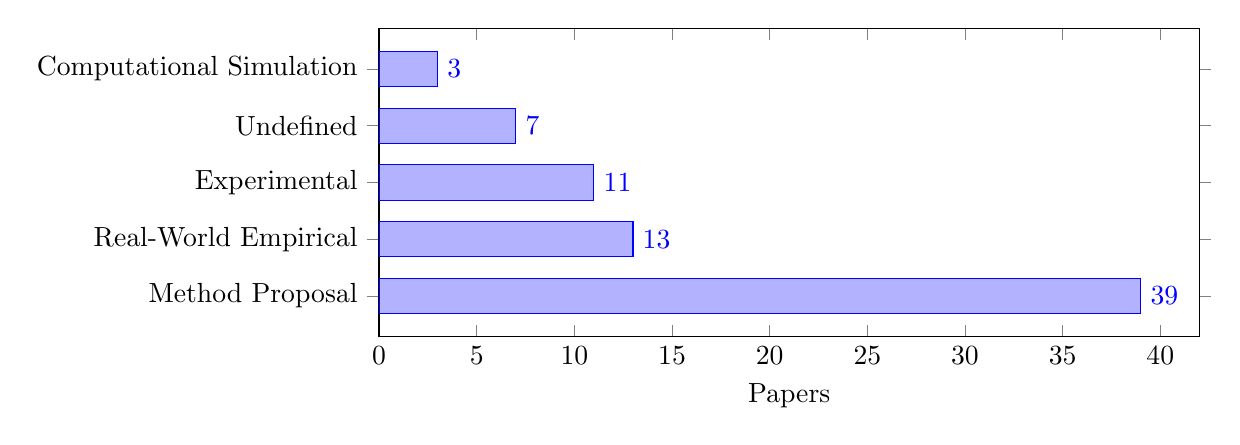
\begin{tikzpicture}
\begin{axis}[
  xbar,
  bar width=0.45cm,
  width=12cm, height=5.5cm,
  xlabel={Papers},
  symbolic y coords={Method Proposal,Real-World Empirical,Experimental,Undefined,Computational Simulation},
  ytick=data,
  xmin=0, xmax=42,
  nodes near coords,
  nodes near coords align={horizontal},
  fill=gray!45,
  draw=black,
  enlarge y limits=0.18,
]
\addplot coordinates {
  (39,{Method Proposal})
  (13,{Real-World Empirical})
  (11,{Experimental})
  (7,{Undefined})
  (3,{Computational Simulation})
};
\end{axis}
\end{tikzpicture}
\caption{Evidence-type distribution in the 73-paper PDF enrichment subset.}
\label{fig:pdf-evidence-dist}
\end{figure}


\section{Discussion}
\label{sec:slr-discussion}

\subsection{Research Gap Identification}
\label{sec:slr-gaps}

The analysis of 2{,}340 screened records and 143 provisionally confirmed primary studies,
together with the criterion coverage patterns, supports five key findings:

\begin{description}

\item[F1: Descriptive Ceiling.]
104 of 143 provisionally confirmed papers (72.7\%) match IC1/IC4a (process mining in SE), but
only 23 (16.1\%) advance to IC3/IC4c (forecasting of process metrics). The
dominant contribution type is discovery or conformance checking, not
predictive analytics or distributional forecasting. This confirms the
descriptive ceiling reported anecdotally in prior surveys.

\item[F2: Event Log Construction Challenge.]
The construction of event logs from heterogeneous software repository sources
appears as a primary challenge across virtually all studies that mention data
collection procedures. The absence of standardized construction frameworks
limits reproducibility and cross-study comparability. The 73-paper enrichment
confirms that most studies still rely on ad hoc joins between issues, commits,
repository events, and pipeline logs rather than on reusable construction
protocols.

\item[F3: Stochastic Integration Gap.]
Only 44 of 143 provisionally confirmed papers (30.8\%) apply stochastic models (IC2/IC4b) to
software processes, and only 17 papers (11.9\%) combine stochastic modeling with
forecasting (IC2 $\cap$ IC3). Markov chains and Monte Carlo simulation are
used extensively in BPM and software reliability engineering, but their
integration with process mining for SDLC forecasting is minimal. This gap is
further evidenced by EC3 being the dominant exclusion reason across both
FT screening rounds ($n \approx 219$, 44.1\% of 497 FT excludes): the
stochastic modeling community has not converged on applying its techniques to
software development process data. The full-paper enrichment leads to the same
conclusion from a different angle: among the 73 analyzed PDFs, only 5 show an
explicit overlap between process mining and stochastic modeling.

\item[F4: Pipeline Fragmentation.]
Studies apply techniques in isolation. The formal composition of a
PM $\rightarrow$ Markov $\rightarrow$ MC $\rightarrow$ ML pipeline with
inter-stage data contracts has not been proposed in the literature for SDLC
contexts. IC combination analysis confirms that multi-criterion papers
(IC4a $+$ IC4b $+$ IC4c $+$ IC4d simultaneously) are effectively absent. The
73-paper reading sheets further show that even when stochastic components are
present, validation usually stops at process analysis, duration estimation, or
simulation, without a downstream learning component.

\item[F5: Process-Derived Features Unexplored.]
ML-based prediction studies in software engineering rely on traditional
features (code metrics, commit characteristics) and rarely incorporate features
derived from process mining (conformance scores, rework counts,
Markov-expected remaining time, path entropy).

\end{description}

These five findings map directly to the five deficits identified in
Section~\ref{sec:gap-analysis}: F1 corresponds to D1 (Descriptive Ceiling),
F3 to D3 (Stochastic Integration Absence), F4 to D5 (Pipeline Fragmentation),
and F5 to D4 (Feature Engineering Void). F2 provides empirical evidence for a
challenge that PATHCAST addresses through Stage~1 (Event Log Construction).


\subsection{Positioning of PATHCAST}
\label{sec:slr-positioning}

Table~\ref{tab:positioning} positions PATHCAST against the integration levels
identified in the current included set.

Because the formal full-text extraction of all 143 provisionally confirmed studies is still
ongoing, Table~\ref{tab:positioning} distinguishes between the
\textit{operational coding} obtained from the 73 locally analyzed PDFs and the
conceptual interpretation of what each level means for PATHCAST.

\begin{table}[htbp]
\centering
\caption{Integration levels in the operationally coded PDF subset and
  PATHCAST positioning.}
\label{tab:positioning}
\small
\setlength{\tabcolsep}{4pt}
\begin{tabular}{c p{6.0cm} c p{3.6cm}}
\toprule
\textbf{Level} & \textbf{Description} & \textbf{Papers}
  & \textbf{Example} \\
\midrule
L0 & Exactly one analytical family is explicit (e.g., only PM, only stochastic, or only contextual analysis)
  & 13 & Contextual or single-technique studies \\
L1 & Two analytical families are present in the same study, but without an explicit reproducible pipeline contract between them
  & 54 & Discovery, conformance, or stochastic analysis without full pipeline closure \\
L2 & A partial bridge between PM and stochastic analysis is explicit, but the workflow remains incomplete or lacks ML closure
  & 6 & Partial bridges such as stochastic conformance or PM + simulation \\
L3 & Unified framework: PM $+$ Markov $+$ MC $+$ ML with formal contracts
  & 0 & \textbf{PATHCAST} \\
\bottomrule
\end{tabular}
\end{table}

PATHCAST is positioned at level L3---the first proposal, to the best of the
author's knowledge, to formally compose process mining, absorbing Markov chain
analysis, Monte Carlo forecasting, and ML enhancement into a single
architecturally specified pipeline applied to SDLC data.


\subsection{Proposed Taxonomy: SPMF}
\label{sec:slr-taxonomy}

Based on the systematic analysis, this review proposes the Software Process
Mining and Forecasting (SPMF) taxonomy with three dimensions:

\begin{description}
\item[Analytical Depth] classifies studies along four levels: L1
  (Descriptive: discovery, conformance), L2 (Diagnostic: bottleneck, rework),
  L3 (Predictive: outcome, remaining time), and L4 (Forecasting:
  distributional, probabilistic).

\item[SDLC Coverage] maps which lifecycle phases are addressed: Requirements
  and Design, Development (coding, commits, PRs), Quality (testing, reviews,
  bugs), Delivery (CI/CD, release), and Operations (incidents, maintenance).

\item[Technique Integration] classifies methodological combination:
  Single (PM only, ML only, MC only), Dual (PM + ML, PM + Markov, Markov + MC),
  and Pipeline (PM $\rightarrow$ Markov $\rightarrow$ MC $\rightarrow$ ML).
\end{description}


\subsection{Research Agenda}
\label{sec:slr-agenda}

The gaps identified motivate four research directions:

\begin{description}
\item[RA1: Standardized Event Log Construction for SDLC.]
  Frameworks for transforming heterogeneous repository data into comparable
  event logs with cross-tool case correlation. Maps to Stage~1 of PATHCAST.

\item[RA2: Process-Aware Stochastic Forecasting.]
  Formal integration of process mining with Markov chains and Monte Carlo
  simulation for distributional SDLC forecasting. Maps to Stages~2--4 of
  PATHCAST.

\item[RA3: Process-Derived Features for ML.]
  Systematic exploration of features derived from process mining for outcome
  prediction. Maps to the ML Enhancement Component of PATHCAST.

\item[RA4: Empirical Benchmarking.]
  Evaluation of forecasting methods on comparable OSS repository datasets with
  temporal hold-out and standardized baselines. Maps to the empirical
  evaluation in Chapter~\ref{ch:evaluation}.
\end{description}


\subsection{Preliminary Implications for Practitioners}
\label{sec:slr-practitioners}

Practitioners developing software measurement programs should note three
preliminary actionable insights from the current included set. First, the availability of
structured event log data in issue tracking systems (Jira, GitHub Issues) is
a prerequisite for process mining; organizations should invest in consistent
workflow state management and transition logging before attempting process
analysis. Second, open-source toolkits (PM4Py, ProM, Disco) suffice for
discovery and conformance checking in most SDLC contexts, as suggested by
the current included studies' tool usage patterns. Third, the stochastic extension
(Markov chains for transition probability estimation, Monte Carlo for
throughput forecasting) requires less infrastructure than typically assumed:
the data already exists in the event logs; the challenge is methodological
composition, not data collection.


\section{Threats to Validity of the SLR}
\label{sec:slr-threats}

\subsection{Construct Validity}

The search strings may exclude studies that use non-canonical terminology.
This threat is mitigated through three mechanisms: the complementary MSR
string, the frontier stochastic-PM string, and snowballing. The 10/10 control
paper recovery provides empirical evidence of high recall.

\subsection{Internal Validity}

LLM-based screening introduces the risk of systematic decision bias. This
threat is addressed by: (i)~structured JSON outputs enabling post-hoc
analysis of rationale patterns; (ii)~human verification of all
\texttt{include} decisions; and (iii)~inter-rater agreement reporting
($\kappa$ target $\geq 0.61$) on a random 20\% sample of all decisions
(validation in progress).

The provisional \texttt{include} set may contain false positives from the T/A
phase: the LLM confirmatory pass at FT level (Round~1) rejected 33 of 108 T/A
\texttt{include} papers (30.6\%), primarily for EC3 (algorithm without SE
evaluation). This false-positive rate is within the expected range for LLM
T/A screening and does not compromise the current provisional synthesis, as
these are caught at the FT phase. The Round~2 screening raised the confirmed
set from 76 to 143 by processing 495 additional \texttt{maybe} papers with
enriched abstracts.

A second internal-validity threat concerns the operational coding introduced
after the PDF-based enrichment (e.g., integration level, reading priority,
RQ coverage, and provisional include/maybe/exclude labels). These labels were
generated as structured decision-support heuristics from the locally available
PDF subset and therefore must not be interpreted as replacements for the
formal screening and data extraction protocol. In this chapter, they are used
only to refine the synthesis, prioritize manual reading, and expose patterns
that remain consistent with the formal PRISMA counts.

\subsection{External Validity}

The review is limited to English-language peer-reviewed publications,
potentially excluding relevant work in other languages or grey literature.
The broad time span (1994--2026) and five-database coverage mitigate
geographic and temporal bias. The deferred high-recall auxiliary corpus
(3{,}441 records from SpringerLink, WoS, Snowball) provides a mechanism for
expansion if gaps in the provisionally confirmed study set are identified.

\subsection{Conclusion Validity}

Preliminary synthesis findings (F1--F5) are based on criterion pattern
analysis rather than full data extraction. Final quantitative claims await
completion of full-text review and the structured data extraction described
in Table~\ref{tab:extraction}. Preliminary findings are explicitly labeled
as such throughout Section~\ref{sec:slr-synthesis}.

The same caution applies to the operationally coded 73-paper PDF subset. Its
value lies in triangulation and prioritization, not in replacing the final
evidence table of the SLR. For that reason, all claims derived from this
subset are explicitly framed as enrichment results and are never used to alter
the formal selection counts.


\section{Chapter Summary}
\label{sec:slr-summary}

This chapter presented a systematic literature review of the intersection of
process mining, stochastic modeling, and machine learning applied to software
process forecasting. The review executed three complementary search strings
across five databases, yielding 8{,}347 records, 5{,}783 after deduplication,
and a 2{,}340-paper operational working set for systematic screening. Title and
abstract screening using a LLM-assisted protocol produced 111 candidate
\texttt{include} decisions and 775 \texttt{maybe} decisions (886 papers for
full-text review).

Full-text LLM screening was executed in two rounds. Round~1 processed the 147
papers with abstracts available at the start of the FT phase (108 T/A
\texttt{include} confirmations + 39 Band~C \texttt{maybe} papers), yielding 76
provisionally confirmed studies. Round~2 followed a cascade abstract-enrichment
step (Semantic Scholar, OpenAlex, CORE, Crossref) that raised abstract
coverage from 16.6\% to 72.6\% (643 of 886 papers), then screened the 495
newly eligible \texttt{maybe} papers, adding 67 further confirmed studies.
The combined result is \textbf{143 provisionally confirmed primary studies},
497 FT excluded, 2 FT pending, and 244 papers still without a FT decision
(pending manual review). The final count is expected in the range of 160--180
upon completion of the remaining manual pass.

Preliminary analysis of the 143 provisionally confirmed studies supports five key findings.
First, the field exhibits a descriptive ceiling: 72.7\% of provisionally confirmed papers
apply process mining to software artifacts (IC1), but only 16.1\% advance to
forecasting of process metrics (IC3) (F1). Second, event log construction from
heterogeneous repository sources is a pervasive challenge (F2). Third, the
integration of stochastic models with process mining for SDLC forecasting is
minimal---only 11.9\% of provisionally confirmed papers combine IC2 and IC3 (F3).
Fourth, no provisionally confirmed study implements a formally composed PM $\rightarrow$
Markov $\rightarrow$ MC $\rightarrow$ ML pipeline for software processes
(F4). Fifth, ML studies in SE rarely incorporate process-derived features
(F5).

To strengthen the synthesis while manual full-text extraction is still in
progress, a 73-paper PDF subset was also operationally coded with SLR-oriented
columns covering decision support, RQ coverage, SDLC phase, integration
level, and reading priority. This enrichment layer reinforced the same
conclusion: the literature is rich in descriptive and diagnostic studies, but
still lacks end-to-end, process-aware forecasting pipelines. In the
operational coding, 54 papers were prioritized for immediate reading, most
papers remained at L1 integration, and no paper reached L3.

These five gaps directly motivate the PATHCAST method presented in
Chapter~\ref{ch:method}. PATHCAST is positioned at integration level~L3 in
the SPMF taxonomy---the first formally specified pipeline to compose all four
technique families into a unified, architecturally specified framework for
SDLC process forecasting.
